\section{Profile selection}
\label{design:profile_selection}

As explained, the purpose of the profile selection functionality is to inform the launcher of which child profile the user wishes to launch the previously selected app with.

\emph{No child selected} in \autoref{fig:state_diagram} shows the state of the launcher when the system is waiting for the user to select a child profile to launch the previously selected app with.
From \emph{No child selected}, there are two transitions:

\begin{enumerate}
	\item select child
	\item quit
\end{enumerate}

\noindent Regardless of the transition taken, the launcher will be brought back to \emph{No app selected}.
The difference is in the side effects of these transitions. \\

\noindent The side effect of the transition \emph{select child}, is the execution of the previously selected app, whereas the transition \emph{quit} unselects the selected app.

The flow chart in \autoref{fig:profileselection_design} shows the steps involved in the profile selection process.

\begin{figure}[!h]
	\centering
	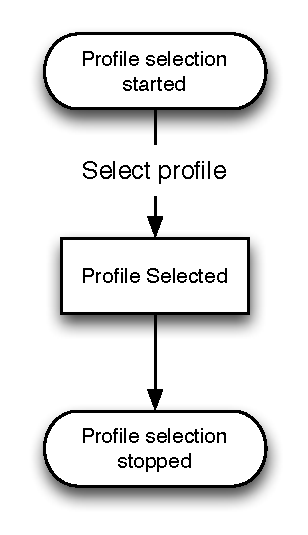
\includegraphics[width=0.6\textwidth]{gfx/profileselect_design.pdf}
	\caption{Flow chart of the profile selection process}
	\label{fig:profileselection_design}
\end{figure}

%The initial state of this feature is to choose which profile the previous selected should be launched as. This is done by clicking on the chosen profile. If the chosen profile is not visible on the screen, it can be needed to scroll through the profiles in order to find it. When the chosen profile is clicked the profile selection process is over.